\documentclass[11pt]{beamer}
\usetheme{PaloAlto}
\usepackage[utf8]{inputenc}
\usepackage[spanish]{babel}
\usepackage{amsmath}
\usepackage{amsfonts}
\usepackage{amssymb}
\usepackage{graphicx}
\graphicspath{{figures/}}
\usepackage{ragged2e}
\usepackage{listings}
\usepackage{xcolor}
\usepackage{hyperref}
\hypersetup{urlcolor=blue}
\logo{
\includegraphics[width=1.4cm]{fac-logo-w}} 
\institute{Facultad de Ciencias \\ Universidad Nacional Autónoma de México} 
\setbeamertemplate{caption}[numbered]
\author[C. Espinosa]{Carlos Espinosa Ponce}
\title{Instalación de CodeBlocks}
\subtitle{Con compilador}

\begin{document}

\begin{frame}
\maketitle    
\end{frame}

\section{Introducción}
\begin{frame}{Editores IDE}
    \begin{block}{Integrated Development Enviroment}
    \justifying
    Los editores IDE (por sus siglas en inglés) son entornos especializados para el desarrollo de software. Tiene herramientas para facilitar la escritura de código y el despliegue de aplicaciones.
    \end{block}
    \justifying
    Existen una gran variedad de IDEs con diferentes características. Además, existen IDEs especializados en un solo lenguaje.
    
    Para el \emph{lenguaje C} existe una amplia selección de IDEs. Uno de ellos es \textbf{CodeBlocks} el cual se caracteriza por incluir un \emph{compilador} de C en su versión para el SO Windows.
\end{frame}

\section{CodeBlocks}
\subsection{Descarga}
\begin{frame}{Descargando CodeBlocks}
    \justifying
\begin{itemize}
    \item Para instalar CodeBlocks necesitamos el instalador de la página oficial.
\end{itemize}
    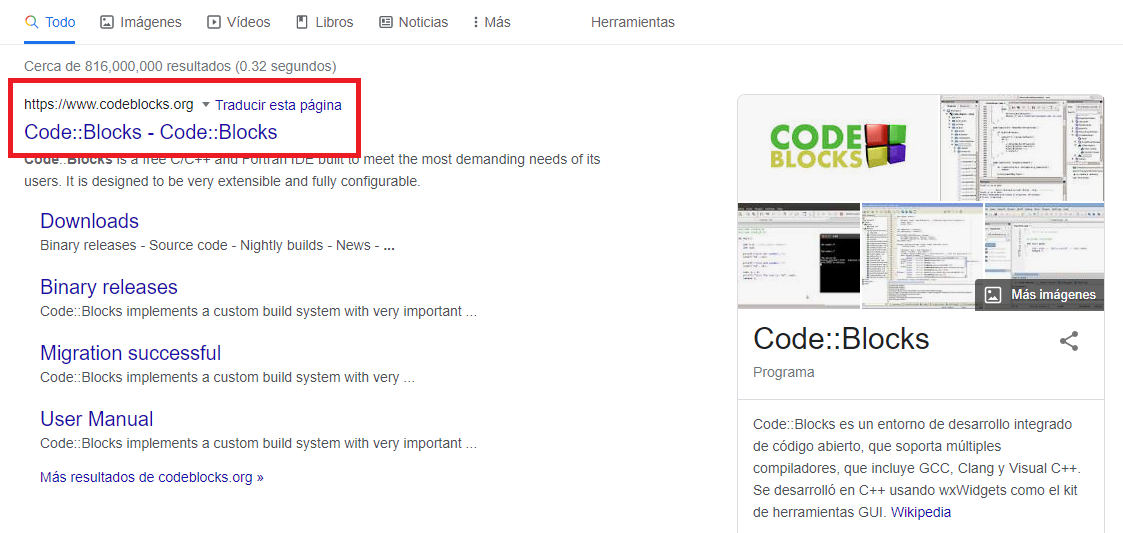
\includegraphics[width=\textwidth]{cb1.png}
\end{frame}

\begin{frame}{Descargando CodeBlocks}
    \justifying
\begin{itemize}
    \item Para instalar CodeBlocks necesitamos el instalador de la página oficial.
\end{itemize}
    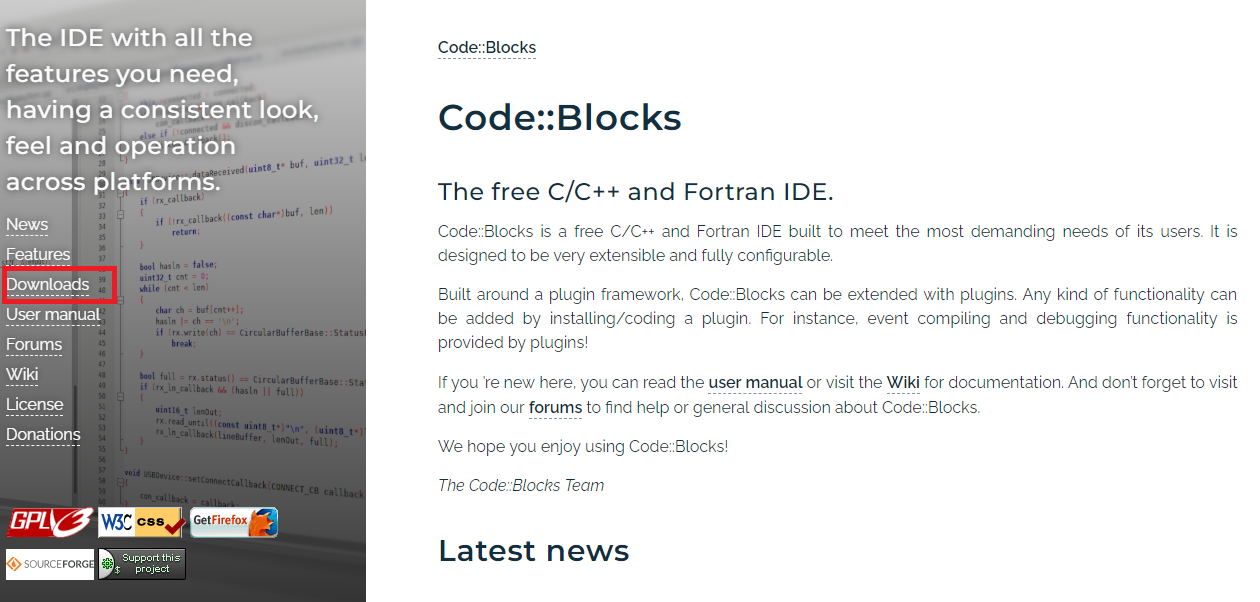
\includegraphics[width=\textwidth]{cb2.png}
\end{frame}

\begin{frame}{Descargando CodeBlocks}
    \justifying
\begin{itemize}
    \item Para instalar CodeBlocks necesitamos el instalador de la página oficial.
\end{itemize}
    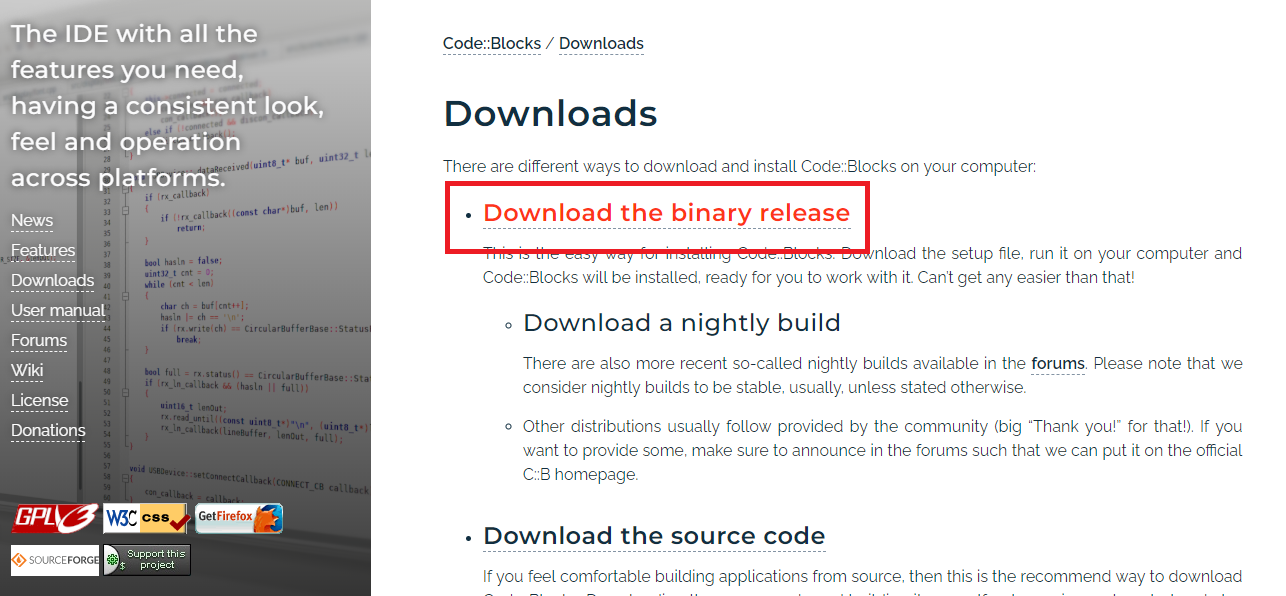
\includegraphics[width=\textwidth]{cb4.png}
\end{frame}

\begin{frame}{Descargando CodeBlocks}
    \justifying
\begin{itemize}
    \item Escogemos el sistema operativo correspondiente.
\end{itemize}
    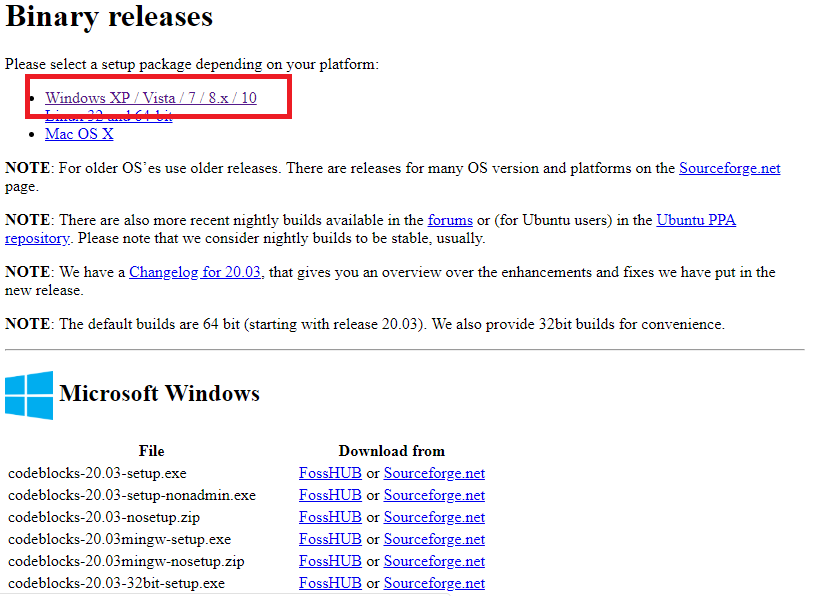
\includegraphics[width=\textwidth]{cb5.png}
\end{frame}

\begin{frame}{Descargando CodeBlocks}
    \justifying
\begin{itemize}
    \item Escogemos el instalador (\textbf{codeblocks-20.03mingw-setup.exe}) y lo descargamos de cualquiera de las dos opciones.
\end{itemize}
    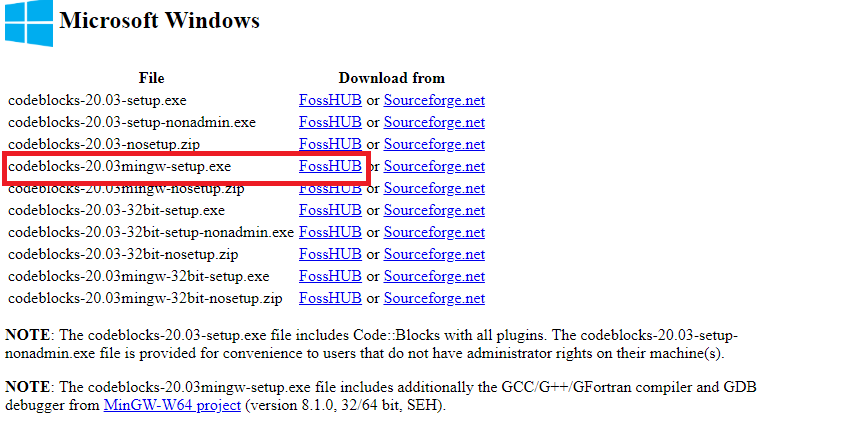
\includegraphics[width=\textwidth]{cb6.png}
\end{frame}
\subsection{Instalación}
\begin{frame}{Instalando CodeBlocks}
    \justifying
    Una vez descargado el instalador, procedemos a ejecutarlo.
    
    \centering
    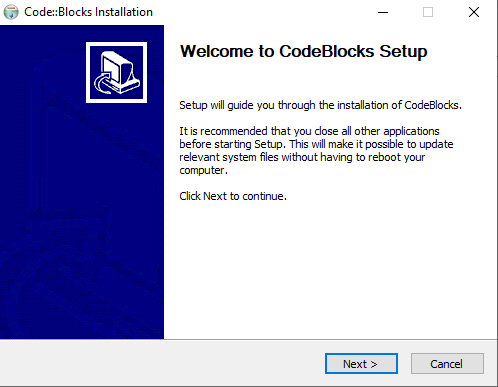
\includegraphics[width=0.75\textwidth]{cb7.png}
\end{frame}
\begin{frame}{Instalando CodeBlocks}
    \justifying
    El proceso de instalación es bastante simple, solo basta dar siguiente, aceptar la licencia...
    
    \centering
    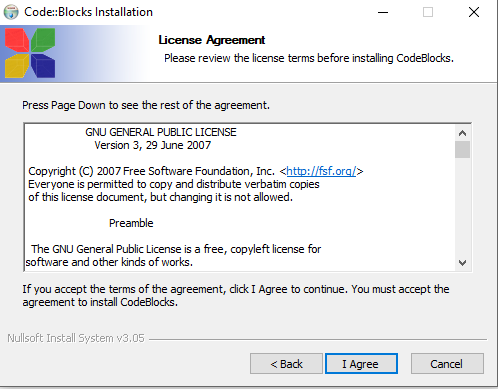
\includegraphics[width=0.75\textwidth]{cb18.png}
\end{frame}
\begin{frame}{Instalando CodeBlocks}
    \justifying
    El proceso de instalación es bastante simple, solo basta dar siguiente, aceptar la licencia y revisar que todo se instale...
    
    \centering
    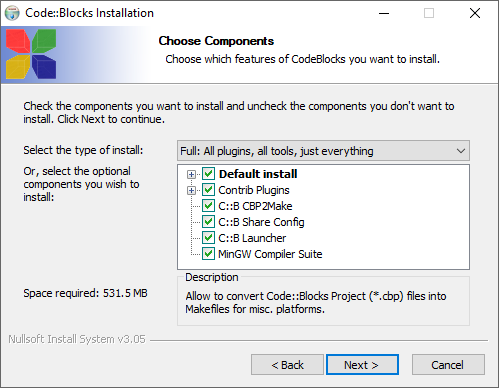
\includegraphics[width=0.75\textwidth]{cb19.png}
\end{frame}
\begin{frame}{Instalando CodeBlocks}
    \justifying
    El proceso de instalación es bastante simple, solo basta dar siguiente, aceptar la licencia y revisar que todo se instale y donde...
    
    \centering
    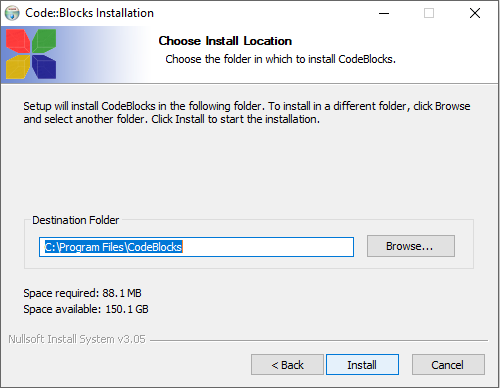
\includegraphics[width=0.75\textwidth]{cb10.png}
\end{frame}
\begin{frame}{Instalando CodeBlocks}
    \justifying
    El proceso de instalación es bastante simple, solo basta dar siguiente, aceptar la licencia y revisar que todo se instale y donde y esperamos.
    
    \centering
    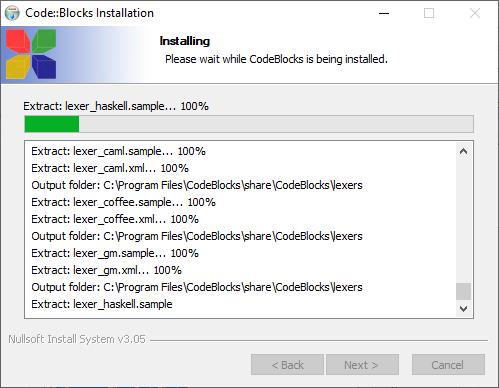
\includegraphics[width=0.75\textwidth]{cb11.png}
\end{frame}
\begin{frame}{Instalando CodeBlocks}
    \justifying
    Cuando termine nos preguntará si queremos iniciar el programa, le damos siguiente y finalizar.
    
    \centering
    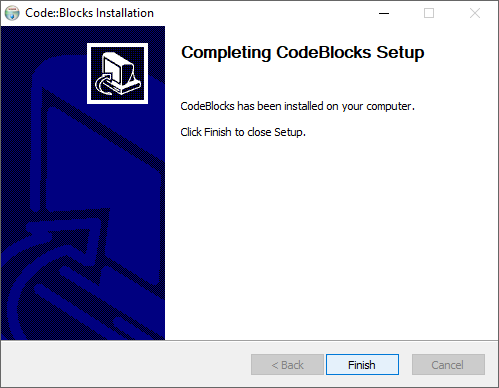
\includegraphics[width=0.75\textwidth]{cb14.png}
\end{frame}
\section{Usando CB}
\begin{frame}{Usando CodeBlocks}
    \justifying
    La primera vez que se abre el programa puede tardar en iniciar y solo ver su logo.
    
    \centering
    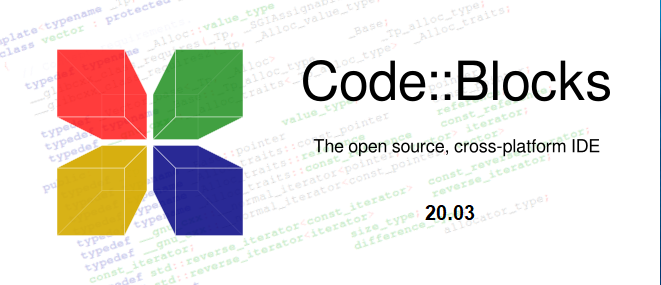
\includegraphics[width=0.75\textwidth]{cb15.png}
\end{frame}
\begin{frame}{Usando CodeBlocks}
    \justifying
    Lo primero que veremos será si queremos hacer que CB sea la aplicación para abrir los archivos de C/C++ (esto es a gusto del usuario.)
    
    \centering
    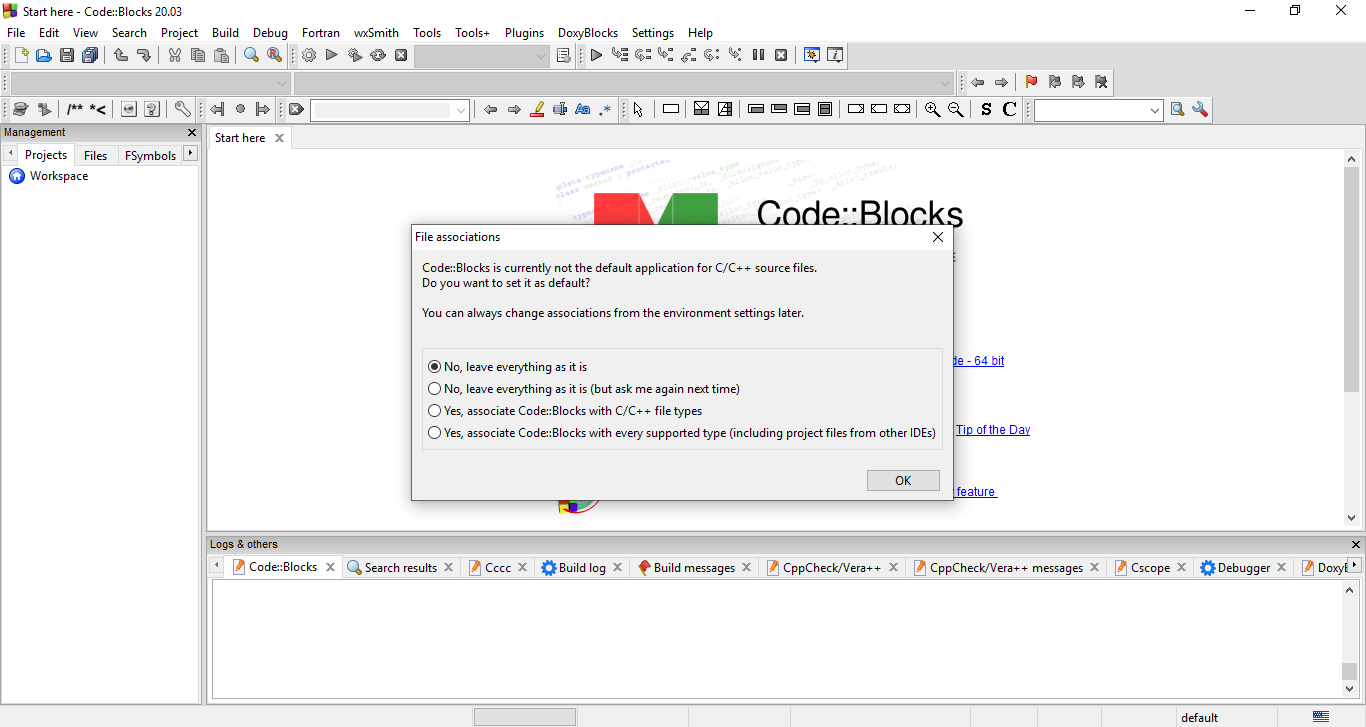
\includegraphics[width=\textwidth]{cb20.png}
\end{frame}
\subsection{Hola mundo}
\begin{frame}{Creando un archivo/proyecto}
    \justifying
    Este tipo de editores se maneja por proyectos. Por lo que crearemos un nuevo proyecto desde el menú archivo (\emph{File} en inglés)
    
    \centering
    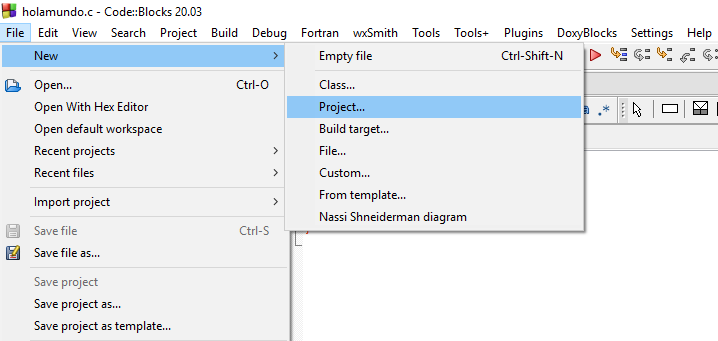
\includegraphics[width=\textwidth]{cb24_1.png}
\end{frame}
\begin{frame}{Creando un archivo/proyecto}
    \justifying
    En la ventana que aparece seleccionamos aplicación de consola (Console Application) y presionamos en el boton \emph{go}.
    
    \centering
    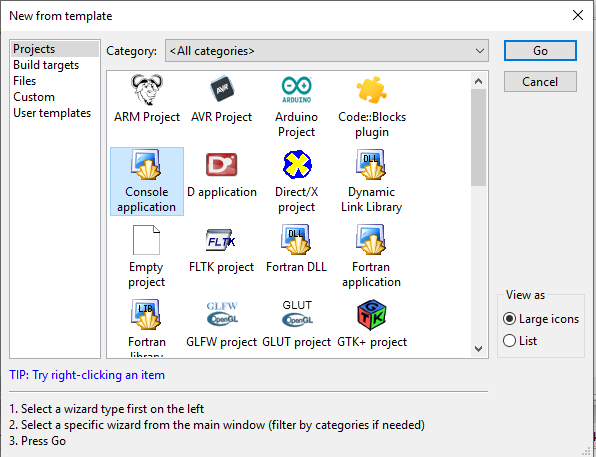
\includegraphics[width=0.75\textwidth]{cb25_1.png}
\end{frame}
\begin{frame}{Creando un archivo/proyecto}
    \justifying
    Se abrirá el \emph{configurador} para este tipo de proyectos.
    
    \centering
    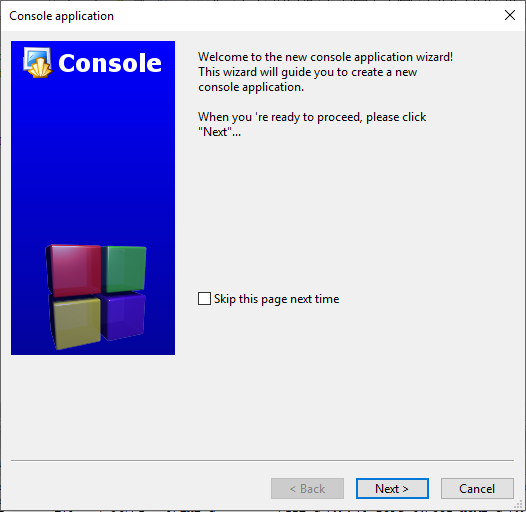
\includegraphics[width=0.75\textwidth]{cb26_1.png}
\end{frame}
\begin{frame}{Creando un archivo/proyecto}
    \justifying
    Seleccionamos el lenguaje a utilizar (en este caso C)
    
    \centering
    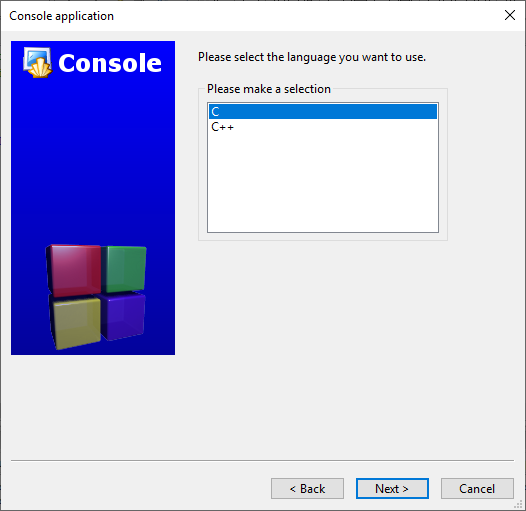
\includegraphics[width=0.75\textwidth]{cb27_1.png}
\end{frame}
\begin{frame}{Creando un archivo/proyecto}
    \justifying
    Definimos el titulo y donde se guardará el proyecto.
    
    \centering
    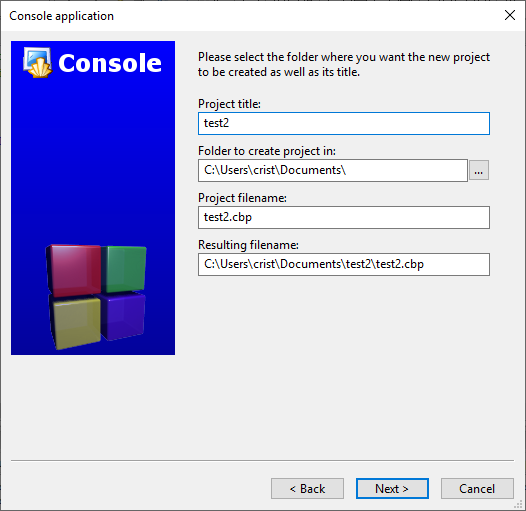
\includegraphics[width=0.75\textwidth]{cb28_1.png}
\end{frame}
\begin{frame}{Creando un archivo/proyecto}
    \justifying
    Se define el compilador por defecto para este proyecto. En este caso será GNU GCC compiler (el que viene incluido en CodeBlocks)
    
    \centering
    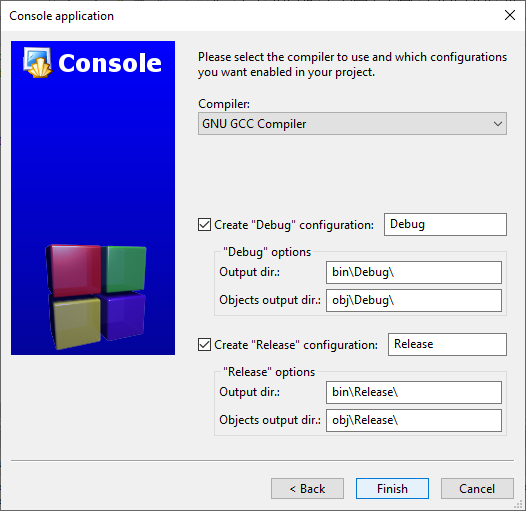
\includegraphics[width=0.75\textwidth]{cb29_1.png}
\end{frame}
\begin{frame}{Creando un archivo/proyecto}
    \justifying
    Del lado izq veremos las carpetas dentro de nuestro proyecto y del lado izquierdo el editor.
    
    \centering
    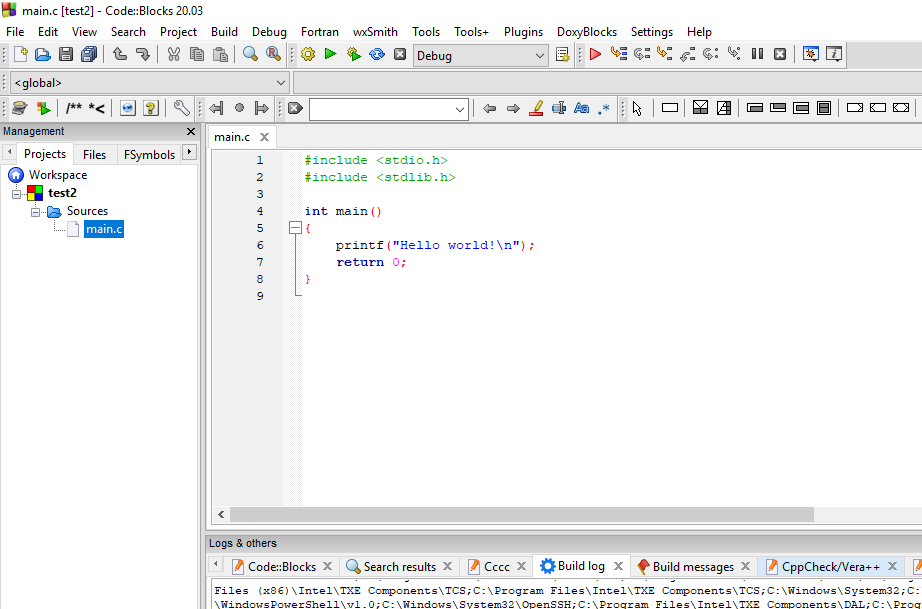
\includegraphics[width=\textwidth]{cb30_1.png}
\end{frame}
\begin{frame}{Creando un archivo/proyecto}
    \justifying
    Para compilar y correr nuestro código usamos el botón que tiene un engrane y un símbolo verde. Veremos un mensaje del compilador en la parte inferior.
    
    \centering
    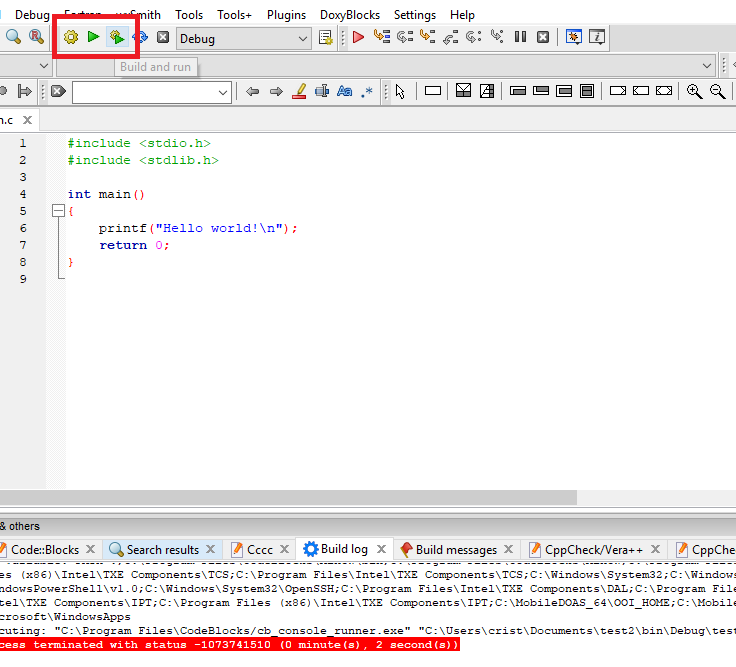
\includegraphics[scale=0.35]{cb31_1.png}
\end{frame}
\begin{frame}{Creando un archivo/proyecto}
    \justifying
    Si la compilación es satisfactoria, se ejecutará en una terminal o consola nuestro programa.
    
    \centering
    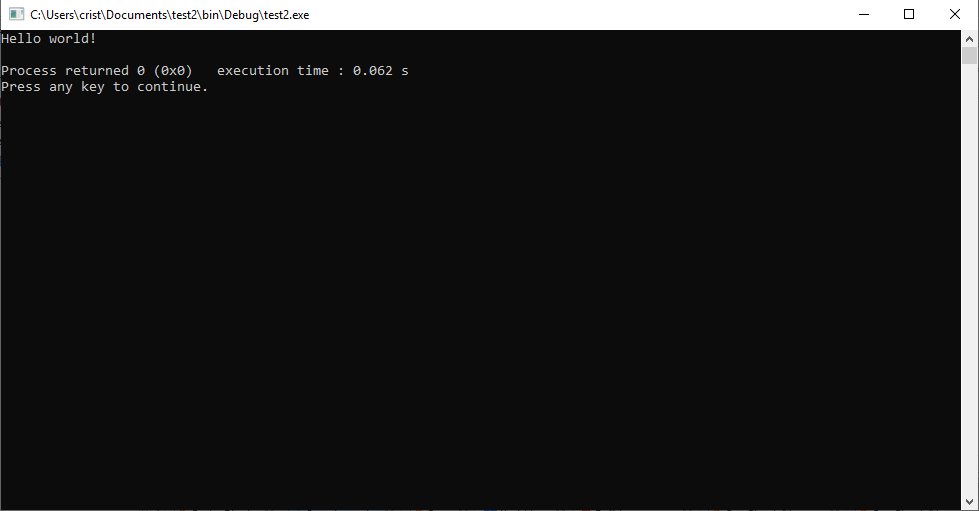
\includegraphics[width=\textwidth]{cb32_1.png}
\end{frame}
\end{document}
